\documentclass[12pt, a4paper]{article}

\usepackage[margin=2.5cm]{geometry}
\usepackage{graphicx}
\usepackage{booktabs}
\usepackage{amsmath}
\usepackage{hyperref}
\usepackage{caption}
\usepackage{subcaption}
\usepackage{float}
\usepackage{microtype}
\usepackage{parskip}
\usepackage{setspace}
\usepackage[numbers]{natbib}

\hypersetup{colorlinks=true, linkcolor=blue, citecolor=blue, urlcolor=blue}

\title{\textbf{Comparative Analysis of Classical and Deep Learning Methods\\
for Satellite Image Classification}\\[0.5em]
\large Machine Learning Final Project Report}

\author{Michelangelo Nardi\\
\small Individual Project. All roles undertaken by the author.}

\date{May 2026}

\begin{document}

\maketitle

% ─────────────────────────────────────────────────────────────────────────────
\section*{Author Responsibilities}
% ─────────────────────────────────────────────────────────────────────────────

This is an individual project. All tasks were undertaken by Michelangelo Nardi, including: conceptualization, data curation, software development, formal analysis, visualization, and writing \cite{niso_credit}.

% ─────────────────────────────────────────────────────────────────────────────
\begin{abstract}
% ─────────────────────────────────────────────────────────────────────────────
Satellite image classification is a critical task in precision agriculture, enabling land-use monitoring, vegetation assessment, and resource management at scale. This paper presents a comprehensive comparative study of classical machine learning and deep learning approaches applied to a four-class satellite image classification task (cloudy, desert, green area, water). Starting from pixel-based features, we evaluate Logistic Regression, Support Vector Machines (SVM), Random Forest, and XGBoost as classical baselines, then progress to a custom Convolutional Neural Network (CNN), and finally fine-tune two pretrained architectures (ResNet18 and EfficientNet-B0) using transfer learning with data augmentation. We further investigate ensemble strategies including soft voting and stacking. Results show a clear performance hierarchy: classical models achieve up to 93.9\% test accuracy, the custom CNN reaches 96.4\%, and transfer learning models exceed 99.6\%. A stacking ensemble attains 99.9\% accuracy on the held-out test set. We discuss the trade-off between model complexity, training cost, and generalization, and analyze the error patterns of the best-performing model.
\end{abstract}

% ─────────────────────────────────────────────────────────────────────────────
\section{Introduction}
% ─────────────────────────────────────────────────────────────────────────────

Remote sensing and satellite imagery have become indispensable tools in modern agriculture. Automated classification of land cover types (vegetation, water bodies, deserts, cloud cover) enables large-scale crop monitoring, drought detection, and irrigation planning \cite{rs_agriculture_review}. Traditional approaches relied on handcrafted spectral indices and rule-based classifiers, but the availability of large annotated datasets and GPU-accelerated computation has made deep learning the dominant paradigm in remote sensing \cite{deep_learning_rs}.

Despite the widespread adoption of deep learning, classical machine learning methods remain practically relevant in settings where labeled data is scarce, computational resources are limited, or model interpretability is required \cite{classical_vs_dl}. A rigorous comparative study bridging both paradigms is therefore valuable, both as an educational exercise and as a practical guide.

This work addresses the following research questions: (1) How do classical machine learning models perform on satellite image classification when operating directly on raw pixel features? (2) Does spatial structure, as exploited by CNNs, provide significant gains over global pixel statistics? (3) Can transfer learning from models pretrained on natural images generalize effectively to satellite imagery? (4) Do ensemble strategies provide meaningful gains over individual models?

We evaluate all models on a common dataset and experimental protocol, enabling a fair and direct comparison across the full spectrum from simple baselines to state-of-the-art transfer learning.

This work builds on feedback received at the proposal and midterm stages. At the proposal stage, feedback indicated that the experimental setup description lacked sufficient detail and that the project timeline was insufficiently specific; the methodology presented here addresses both points with a precise experimental protocol and clearly staged model development. At the midterm stage, feedback noted that progress on ML models was incomplete, as transfer learning had not yet been implemented and ensemble strategies were absent; both are fully realized in this final report.

% ─────────────────────────────────────────────────────────────────────────────
\section{Materials and Methods}
% ─────────────────────────────────────────────────────────────────────────────

\subsection{Dataset}

We use the Satellite Image Classification dataset from Kaggle \cite{kaggle_dataset}, which contains RGB satellite images organized into four semantic classes: \textit{cloudy}, \textit{desert}, \textit{green\_area}, and \textit{water}. The raw dataset presents two challenges: (1) class imbalance, where the desert class contains only 1,131 images (with 36 duplicates) versus 1,500 images in each other class; and (2) resolution inconsistency, where cloudy and desert images are 256$\times$256 pixels while green\_area and water images are 64$\times$64 pixels.

Visual inspection confirms that the four classes are strongly separable by color and texture: cloudy images exhibit gray-white tones with low saturation, desert images display warm ochre hues with granular texture, green\_area images show dark green uniform regions, and water images appear as dark blue-gray surfaces (Figure~\ref{fig:samples}).

\begin{figure}[H]
    \centering
    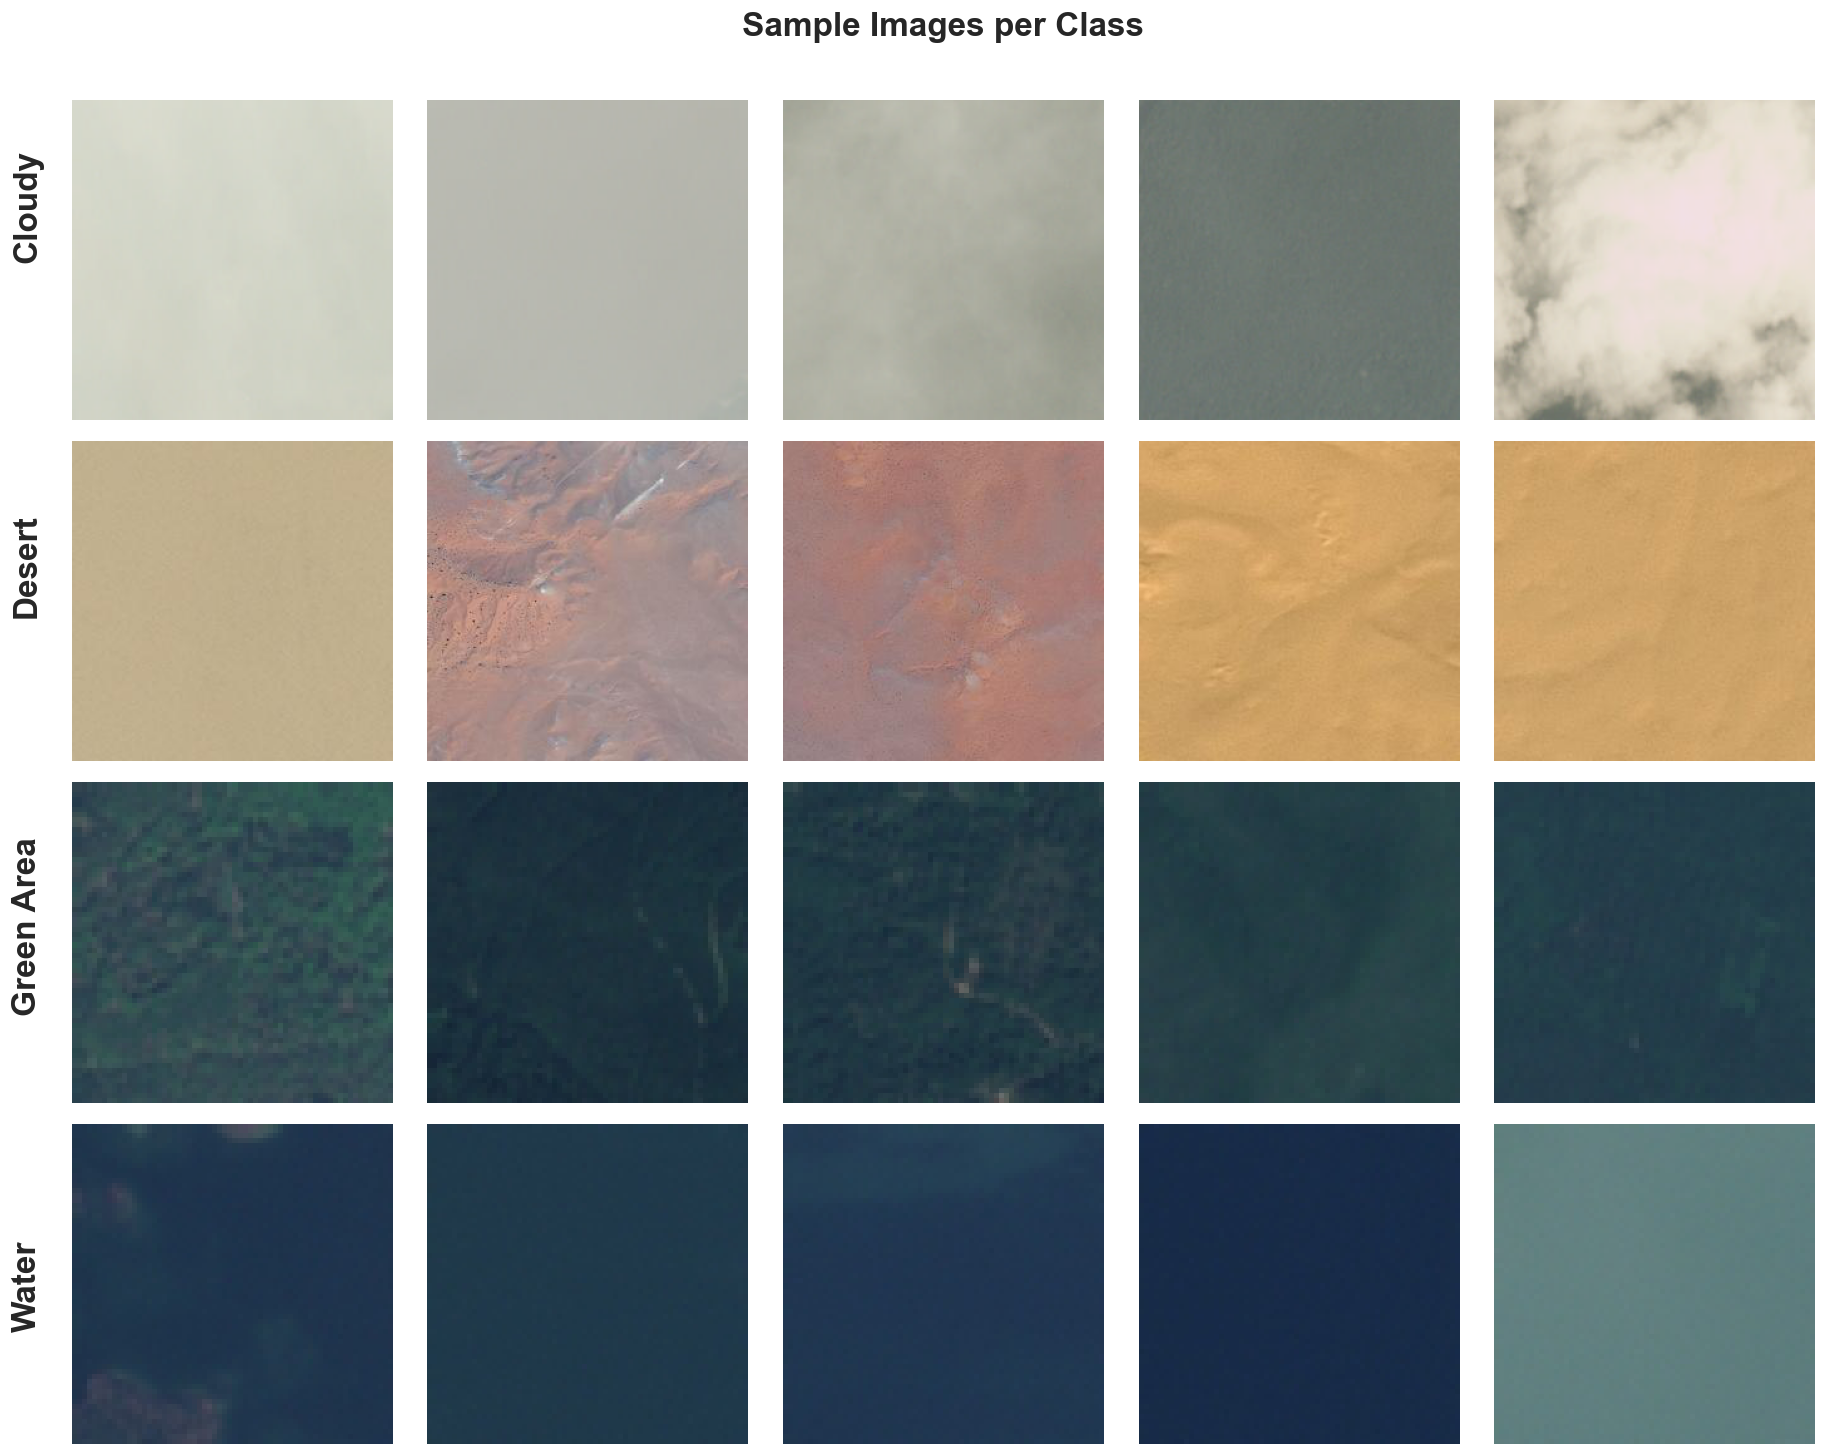
\includegraphics[width=0.7\linewidth]{results/../saved_images/sample images per class 2.png}
    \caption{Representative samples from each of the four classes. Strong color and texture differences are visible across classes, motivating the use of both pixel-based and spatial models.}
    \label{fig:samples}
\end{figure}

\subsection{Preprocessing}

To address the dataset challenges, we apply the following preprocessing pipeline:

\begin{enumerate}
    \item \textbf{Duplicate removal}: 36 duplicate desert images identified via MD5 hashing are removed.
    \item \textbf{Patch extraction}: 256$\times$256 desert and cloudy images are split into non-overlapping 64$\times$64 patches, yielding additional samples and standardizing resolution across all classes.
    \item \textbf{Class balancing}: Each class is capped at 1,500 images, resulting in a balanced dataset of 6,000 images total.
    \item \textbf{Normalization}: Pixel values are scaled to $[0, 1]$ by dividing by 255.
    \item \textbf{Train/test split}: An 80/20 stratified split yields 4,800 training and 1,200 test images (300 per class in each split).
\end{enumerate}

For classical machine learning, images are further flattened into 12,288-dimensional feature vectors ($64 \times 64 \times 3$). Distance-based models (Logistic Regression, SVM) receive standardized features (zero mean, unit variance) via \texttt{StandardScaler}.

\subsection{Experimental Protocol}

We follow a two-stage model development strategy. In the first stage, all candidate models are evaluated via a single-split experiment (80/20 of the training data) to identify promising configurations. In the second stage, the strongest models undergo full 5-fold stratified cross-validation on the training set for hyperparameter tuning. The held-out test set is reserved exclusively for final evaluation after all model selection decisions are made, preventing any optimistic bias from test-set leakage.

Metrics reported are accuracy and macro-averaged F1-score, chosen because the dataset is balanced and all classes are of equal importance.

\subsection{Classical Machine Learning Models}

All classical models operate on the flattened 12,288-dimensional pixel representation. Four model families are evaluated:

\textbf{Logistic Regression} serves as a linear baseline. Given the high dimensionality (12,288 features for 4,800 samples), strong L2 regularization ($C=0.1$) is applied to prevent overfitting. This model captures only global linear relationships between pixel intensities and class labels.

\textbf{Support Vector Machine (SVM)} with an RBF kernel is well-suited to high-dimensional feature spaces and can model non-linear class boundaries. We use $C=10$ selected via single-split tuning. The RBF kernel implicitly maps inputs to an infinite-dimensional space, allowing separation of complex distributions.

\textbf{Random Forest} is an ensemble of 100 decision trees trained with bootstrap aggregation. It is parameter-efficient, naturally handles non-linear interactions, and is robust to irrelevant features. 5-fold cross-validation yields $94.1\% \pm 1.1\%$ accuracy, confirming stable generalization.

\textbf{XGBoost} is a gradient boosting implementation with $n\_estimators=100$, $learning\_rate=0.1$, $max\_depth=6$, and column/row subsampling at 0.8. It sequentially corrects residual errors and typically outperforms Random Forest on tabular data, though the advantage is smaller here due to the spatial structure of the features being lost in flattening.

\subsection{Deep Learning Models}

\textbf{Simple fully-connected neural network (NN):} A three-hidden-layer MLP (12288→512→256→128→4) with ReLU activations and dropout ($p=0.3$) applied after each layer. This model treats the image as an unordered set of pixel values, ignoring spatial structure. Trained with Adam ($lr=10^{-3}$), batch size 32, and early stopping (patience=10).

\textbf{Custom CNN:} A three-block convolutional network with channels 3→32→64→128, each block consisting of Conv2d (3$\times$3, padding 1) → BatchNorm2d → ReLU → MaxPool2d(2$\times$2) → Dropout2d. The spatial dimensions reduce from 64$\times$64 to 8$\times$8 before a fully-connected head (128$\times$8$\times$8→256→4) with dropout ($p=0.2$). Trained with AdamW ($lr=10^{-3}$, weight decay $10^{-4}$), ReduceLROnPlateau scheduler, and early stopping (patience=10). This architecture explicitly models local spatial patterns and is our strongest from-scratch model.

\subsection{Transfer Learning with Data Augmentation}

Transfer learning leverages weights pretrained on ImageNet \cite{imagenet} to provide strong visual feature extractors without requiring large satellite-specific training sets. We evaluate two architectures:

\textbf{ResNet18} \cite{resnet}: An 18-layer residual network. The final fully-connected layer is replaced with a linear layer mapping 512 features to 4 classes.

\textbf{EfficientNet-B0} \cite{efficientnet}: A compound-scaled network optimized for accuracy/efficiency trade-offs. The classifier head is replaced with a linear layer mapping 1,280 features to 4 classes.

Both models are fine-tuned in two phases. In Phase 1 (10 epochs), only the new classification head is trained with Adam ($lr=10^{-3}$), allowing it to adapt to the new class space before gradients flow into the backbone. In Phase 2 (up to 30 epochs), all layers are unfrozen and fine-tuned with AdamW ($lr=10^{-4}$, weight decay $10^{-4}$) and ReduceLROnPlateau scheduling. Early stopping (patience=8) prevents overfitting.

Training applies data augmentation: random horizontal and vertical flips, random rotation ($\pm 15°$), and color jitter (brightness, contrast, saturation $\pm 0.2$). Augmentation is applied only during training; validation and test images use only the HWC→CHW tensor conversion. Since images are already normalized to $[0,1]$, ImageNet normalization statistics are not applied.

\subsection{Ensemble Methods}

Three ensemble strategies are evaluated using five base models: Logistic Regression, SVM, Random Forest, XGBoost, and ResNet18 (the best individual model overall).

\textbf{Soft voting}: Class probabilities from multiple models are averaged and the argmax is taken. We evaluate four variants: (a) DL-only, combining CNN, ResNet18, and EfficientNet-B0; (b) classical-only, combining Random Forest and SVM; (c) all-model, combining all five base models; and (d) best-DL plus best-classical, combining ResNet18 and Random Forest.

\textbf{Hard voting}: Majority class label across the predictions of all five base models.

\textbf{Stacking}: A Logistic Regression meta-learner is trained on the concatenated probability vectors (20 features = 5 models $\times$ 4 classes) produced by all five base models on the training set. Test predictions use the same base models to generate meta-features for the meta-learner.

% ─────────────────────────────────────────────────────────────────────────────
\section{Results and Discussion}
% ─────────────────────────────────────────────────────────────────────────────

\subsection{Overall Performance}

Table~\ref{tab:results} summarizes test-set accuracy and macro F1 for all models. Figure~\ref{fig:comparison} visualizes the performance hierarchy.

\begin{table}[H]
\centering
\caption{Test-set performance of all models, sorted by accuracy. All results are on the held-out test set of 1,200 images (300 per class).}
\label{tab:results}
\begin{tabular}{llcc}
\toprule
\textbf{Category} & \textbf{Model} & \textbf{Accuracy} & \textbf{Macro F1} \\
\midrule
Ensemble     & Stacking (LR meta-learner on all 5 models) & 0.9992 & 0.9992 \\
Ensemble     & Soft Vote (CNN + ResNet18 + EfficientNet-B0)& 0.9983 & 0.9983 \\
Ensemble     & Soft Vote (all 5 base models)              & 0.9983 & 0.9983 \\
Ensemble     & Soft Vote (ResNet18 + Random Forest)       & 0.9983 & 0.9983 \\
Transfer DL  & ResNet18                       & 0.9975 & 0.9975 \\
Transfer DL  & EfficientNet-B0                & 0.9967 & 0.9967 \\
Ensemble     & Hard Vote (all 5 base models)              & 0.9717 & 0.9716 \\
Custom DL    & CNN (3-block)                  & 0.9642 & 0.9642 \\
Classical    & XGBoost ($n=100$)              & 0.9392 & 0.9393 \\
Classical    & Random Forest ($n=100$)        & 0.9383 & 0.9384 \\
Classical    & SVM (RBF, $C=10$)              & 0.9225 & 0.9224 \\
Custom DL    & Simple NN (MLP)                & 0.8558 & 0.8540 \\
Classical    & Logistic Regression ($C=0.1$)  & 0.8325 & 0.8313 \\
\bottomrule
\end{tabular}
\end{table}

\begin{figure}[H]
    \centering
    \includegraphics[width=0.85\linewidth]{results/final_model_comparison.png}
    \caption{Test-set accuracy and macro F1 across all models. The performance gap between classical tree-based methods and transfer learning models exceeds 6 percentage points.}
    \label{fig:comparison}
\end{figure}

\subsection{Classical Machine Learning}

Classical models achieve competitive performance despite operating on raw 12,288-dimensional pixel vectors. The linear baseline (Logistic Regression, 83.3\%) confirms that the four classes are partially linearly separable, a consequence of the strong color signatures visible in the data. SVM with an RBF kernel improves substantially to 92.3\%, demonstrating that non-linear boundaries matter even for color-dominant features.

Random Forest and XGBoost perform comparably (93.8\% and 93.9\%), both outperforming SVM. Gradient Boosting was also evaluated but abandoned in favor of XGBoost due to its significantly longer training time for equivalent accuracy.

The performance ceiling of classical models is around 94\%. All of these models treat each pixel independently, discarding spatial relationships between adjacent pixels. The confusion patterns (Figure~\ref{fig:classical_cm}) reveal that the primary source of error is confusion between \textit{green\_area} and \textit{water}, two classes that share similar dark, low-saturation tones under certain lighting conditions.

\begin{figure}[H]
    \centering
    \includegraphics[width=\linewidth]{results/classical_models_confusion_matrices.png}
    \caption{Normalized confusion matrices for all four classical models on the held-out test set. Green\_area and water are the most commonly confused class pair across all models.}
    \label{fig:classical_cm}
\end{figure}

\subsection{Custom Deep Learning Models}

The simple MLP (85.6\%) performs worse than the best classical models despite being a neural network, because it also operates on flattened pixel vectors and lacks the inductive bias of convolutional operations. This result highlights that the \textit{depth} of a model alone is insufficient; the appropriate \textit{architectural inductive bias} is what matters.

The custom CNN substantially improves on all baselines, reaching 96.4\% accuracy. Training curves (Figure~\ref{fig:cnn_curves}) show that validation accuracy converges smoothly with no signs of severe overfitting, attributable to BatchNorm and dropout regularization. The CNN exploits local spatial patterns (edges, textures, color gradients) that are informative for satellite scene classification even at 64$\times$64 resolution. The 2.5 percentage point improvement over the best classical model directly quantifies the value of spatial feature learning for this task.

\begin{figure}[H]
    \centering
    \begin{subfigure}[b]{0.48\linewidth}
        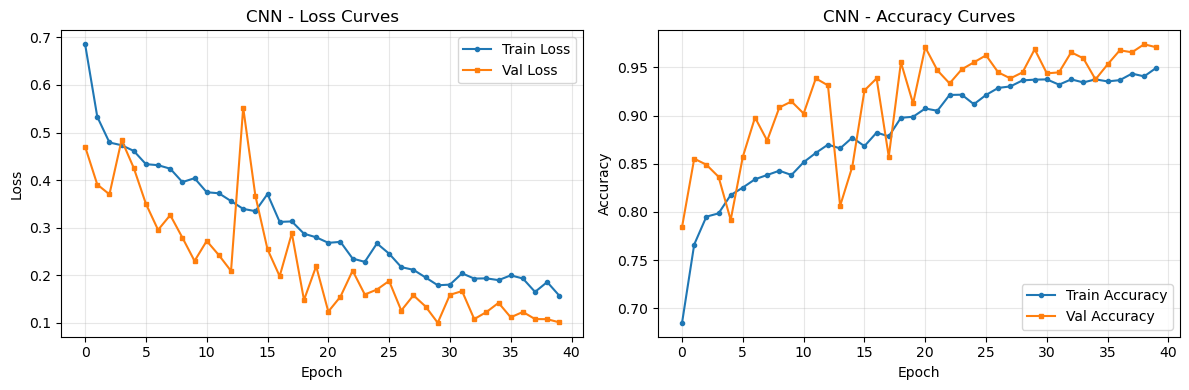
\includegraphics[width=\linewidth]{results/cnn_training_curves.png}
        \caption{Custom CNN}
    \end{subfigure}
    \hfill
    \begin{subfigure}[b]{0.48\linewidth}
        \includegraphics[width=\linewidth]{results/resnet18_training_curves.png}
        \caption{ResNet18 (two-phase fine-tuning)}
    \end{subfigure}
    \caption{Training and validation loss/accuracy curves. The ResNet18 curves show the head-only phase followed by full fine-tuning, with validation accuracy exceeding 99\% within the fine-tuning phase.}
    \label{fig:cnn_curves}
\end{figure}

\subsection{Transfer Learning}

Both ResNet18 (99.75\%) and EfficientNet-B0 (99.67\%) dramatically outperform all from-scratch models. ResNet18 makes only 3 errors on the 1,200-image test set; EfficientNet-B0 makes 4. This near-perfect performance is remarkable given that both models were pretrained on ImageNet, a dataset of natural photographs containing no satellite imagery.

The two-phase fine-tuning strategy is critical: training only the head first allows the model to adapt its output distribution to the new classes before gradients flow into the pretrained backbone, preventing destructive updates to the learned feature representations. Data augmentation further improves robustness by exposing the model to geometric and photometric variations common in real satellite captures.

The validation confusion matrices (Figure~\ref{fig:tl_cm}) confirm that even the hardest class pair (\textit{green\_area} vs.\ \textit{water}) is nearly perfectly resolved, a capability that eluded all classical models and the custom CNN.

\begin{figure}[H]
    \centering
    \includegraphics[width=0.75\linewidth]{results/transfer_learning_val_confusion_matrices.png}
    \caption{Validation-set confusion matrices for ResNet18 and EfficientNet-B0. Both transfer learning models resolve nearly all inter-class confusions, including the green\_area/water pair that posed the greatest challenge to classical models.}
    \label{fig:tl_cm}
\end{figure}

\subsection{Ensemble Methods}

Soft-voting ensembles that include the transfer learning models achieve 99.83\% accuracy. The stacking ensemble reaches 99.92\%, the highest overall, by learning optimal combination weights via the meta-learner.

Interestingly, hard voting underperforms (97.2\%) relative to soft voting. This is because hard voting discards probability calibration information: when one model is highly confident and the others weakly disagree, hard voting can override the confident correct prediction.

The classical-only ensemble (93.3\%) does not outperform the best individual classical model (XGBoost, 93.9\%), suggesting that RF and XGBoost make similar errors that averaging cannot resolve.

\subsection{Per-Class Performance}

Figure~\ref{fig:perclass} shows the macro F1-score broken down by class for each individual model. The pattern is consistent across all models: \textit{cloudy} and \textit{desert} are classified with near-perfect precision and recall even by the weakest models, while \textit{green\_area} and \textit{water} are systematically harder. Transfer learning models achieve uniform performance across all four classes, closing the gap on the two difficult classes entirely.

\begin{figure}[H]
    \centering
    \includegraphics[width=0.85\linewidth]{results/final_perclass_f1_heatmap.png}
    \caption{Per-class F1-score heatmap for all individual models. Warmer colors indicate higher F1. The green\_area and water classes are consistently the most challenging, while cloudy and desert are reliably classified across all model families.}
    \label{fig:perclass}
\end{figure}

\subsection{Error Analysis}

Figure~\ref{fig:errors} shows representative misclassified images from the best-performing model (ResNet18, 3 errors on 1,200 test images). All errors are confusions between \textit{green\_area} and \textit{water}: water bodies with textured surfaces are misclassified as green area, and dark vegetation patches under overcast conditions are misclassified as water. These are visually ambiguous cases where the distinguishing cues (surface texture, color saturation) are weak or absent. Notably, the other two classes (cloudy and desert) are never confused by the best model, consistent with their strong and distinctive visual signatures.

\begin{figure}[H]
    \centering
    \includegraphics[width=0.85\linewidth]{results/error_analysis_misclassified.png}
    \caption{Misclassified test images from ResNet18. All errors are confusions between \textit{green\_area} and \textit{water}, the two visually closest classes in the dataset.}
    \label{fig:errors}
\end{figure}

\subsection{Discussion of Limitations}

Several limitations should be acknowledged. First, all images are at 64$\times$64 resolution, which discards fine-grained spatial detail present in higher-resolution satellite data. Second, the dataset contains only four broad land-cover categories; operational agricultural systems typically require finer granularity (e.g., distinguishing crop types within the green area class). Third, transfer learning from ImageNet may not generalize equally well to multi-spectral or hyperspectral satellite data, where channels beyond RGB carry critical information. Finally, the near-perfect performance of transfer learning models may partly reflect the relative simplicity of the task (strong color and texture discriminability), and results on more challenging remote sensing benchmarks may differ substantially.

% ─────────────────────────────────────────────────────────────────────────────
\section{Conclusion}
% ─────────────────────────────────────────────────────────────────────────────

This paper presented a systematic comparison of classical machine learning and deep learning methods for satellite image classification across four land-cover categories. Classical tree-based models (Random Forest, XGBoost) achieve approximately 94\% accuracy and represent an effective solution when computational resources are limited. The custom CNN improves this to 96.4\% by exploiting spatial structure. Transfer learning with ResNet18 and EfficientNet-B0 achieves near-perfect accuracy (>99.6\%), with a stacking ensemble reaching 99.9\%.

The key insight is that the performance gains from classical models to the custom CNN to transfer learning correspond to increasing amounts of learned spatial hierarchy: from pixel-level global statistics, to locally-learned convolution filters, to deep hierarchical representations pretrained on millions of images. For the specific problem of satellite image classification at 64$\times$64 resolution with strong color and texture cues, transfer learning is the clear practical recommendation.

Future work could extend this study to multi-spectral imagery, finer land-cover categories, and larger-scale datasets such as EuroSAT \cite{eurosat} or BigEarthNet \cite{bigearthnet}, where the relative advantages of different approaches may differ substantially.

% ─────────────────────────────────────────────────────────────────────────────
\bibliographystyle{ieeetr}
\bibliography{references}
% ─────────────────────────────────────────────────────────────────────────────

\end{document}
